\section{Testing, Cleaning and Commissioning} \label{sec:Testing}\label{sec:Commissioning}
Testing of CALIS has been performed at FNAL in the second half of August and first half of September 2014. CALIS was installed in a building with the high bay, on a high platform, so that the full length deployment tests could be performed. The tests are repeated at LNGS prior to cleaning the system, and some validation tests are foreseen at the time of installation in CRH.  Several different tests have been conducted:
\begin{itemize}


\item{Light covers on the view ports}
Light tightness of the whole system

All viewports have  very tightly fitting covers. Additionally, the main viewport cover will additionally be held in place with clamps to avoid any possibility of accidently exposing the LSV to excessive amount of light. 



 \item{Motor controls debugging}

    LabView interface with the motor controls has been verified and responds to all commands (starting/stopping of vertical deployment) as expected.  Motor current can be read from the GUI and shows opposite signs if motor is rotating in one vs the other direction as an additional sign of the  motion direction.

\item{\bf Vertical (z) position accuracy and repeatability}
{\bf Procedure:} As a first step in testing the reproducibility of the z position as a function of step position,
a baseline relationship between step number and vertical displacement was determined. First, the distance
from the floor to the bottom of the pig was measured using a laser ranger, starting from what was found
to be the lowest pig position (fully deployed). The bottom of the pig was covered with tape to serve as a
target for the laser ranger. After this first measurement, the pig was raised, stopping approximately once
every minute to record the step position and measure the corresponding z distance, until it reached the home position (fully retracted). Subsequently, in the following test runs, the pig was again sent to each of these steps, the z position was measured with the laser ranger, and all values recorded. After 2 runs in which every step which had been recorded in the baseline was measured, it was realized that recording so many data points would require several weeks to complete the testing. The number of data points was then cut in half for 4 runs, and cut in half again for the remaining 24 runs for a total of 31 runs.

{\bf Results:} The vertical displacement of the pig was found to be extremely consistent, with no apparent
drift due to slippage or any other effect. The average uncertainty of each z coordinate was found to range
between 1-2\,mm, numbers consistent with the uncertainty of the laser ranger and the unevenness of the tape on the bottom of the pig. Fig.~\ref{fig:z_test} shows the correspondence between the z position and stepper motor count exibiting a smooth function with no visible variation of the points from the fit. No measurable slippage of the cables or accumulated offset of the stepper motor count and z position was observed during the repeated tests.

\begin{figure}[htbp]
 \centering
 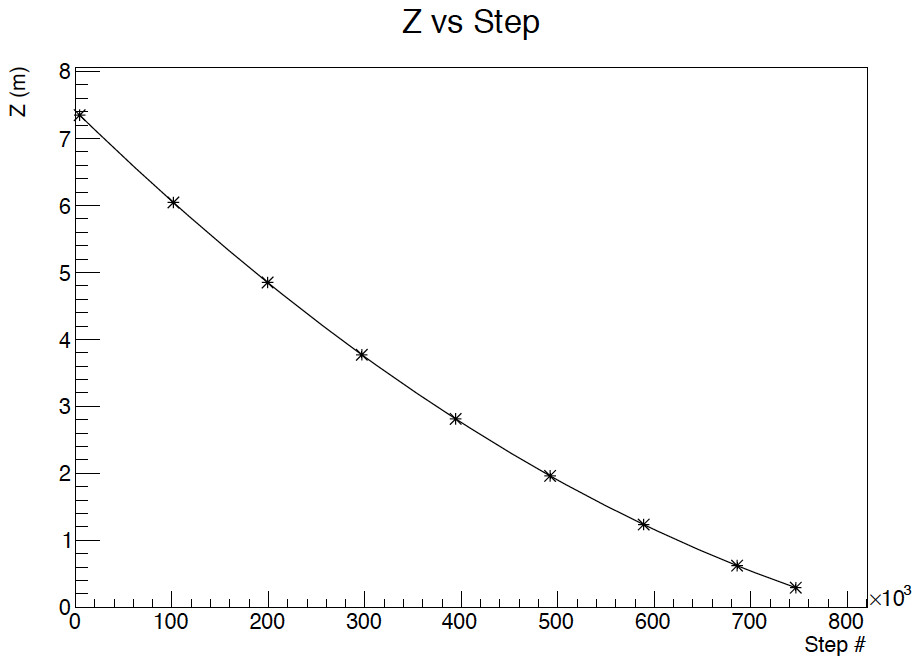
\includegraphics[width=3.2in]{Figures/Z_positioning_test}
 \caption{Plot of the z position of the pig vs the step position of the motor.}
 \label{fig:z_test}
\end{figure}


\item{\bf Lateral motion during depoyment}

The pig is deployed at a very low speed, barely visible to the naked eye. It takes about 30 minutes to deploy the system from its home position to the level of the TPC, approximetely 7\,m below. As a result, there is a negligible level of lateral motion during vertical motion at the level of 2-3\,mm. The motor has a very slow acceleration (both positive and negative) that eliminates any visible jitter at the beginning or at the end of the motion.

\item{\bf Articulation tests}

{\bf Procedure:} Arm is articulated using a manually operated hand wheel.  The arm is articulated to 90$^{\circ}$ every time. This corresponds to a different reading of the dial connected to the hand wheel for different z-position. The second calibration table required, gives correspondence between the z height and required reading on the dial to articulate to 90$^{\circ}$. 

In order to verify the consistency of articulating to the same rotation angle of 90$^{\circ}$ at all needed positions,  full articulation of the arm at different z positions was tested. For this test at Fermi lab, two vertical positions were chosen: one approximately at the center of the cryostat mock-up, and one at the lowest known position of the pig. At each position, the arm was articulated and
the required angle recorded. In order to ensure that the arm was fully articulated, a level was placed on the
arm and required to be horizontal. Additionally, the vertical displacement of the pig was measured before articulating the arm, while the arm was articulated and after the arm was again vertical. Between runs, the
pig was sent all the way back to the home position to simulate the actual deployment conditions as closely as possible. The process was repeated 10 times  (10 runs) to check consistency of articulation among independent runs.

{\bf Results:} During driving the pig up and down through the whole length of the cable, it was noticed that the arm did not return to a perfectly vertical position, which was especially noticeable when the pig was in the home position. To document this, photos were taken each time the arm was de-articulated and when it was in the home position. The hand wheel was renormalized to zero several times, but this offset continued to reappear. It did not seem to progress, however, and remained at approximately the same angle, as can be seen from the photographs in Fig.~\ref{fig:art_offset1}, Fig.~\ref{fig:art_offset2}, Fig.~\ref{fig:art_offset3} and Fig.~\ref{fig:art_offset4}. In all tested cases, offset was relatively small and did not create a problem for retracting the pig inside the lower assembly pipe and to the home posiiton. 

 It was noted that some of this offset was due to the fact that the pig is allowed to swing freely. When articulating the arm, one cable on one side of the pig is raised. This causes the pig to also slightly move in the direction of the articulation. After the
arm is dearticulated, the arm returned to vertical according to the hand wheel, but not according to visual
inspection and use of a level. Part of the offset is because the pig moved in the direction of articulation and
during dearticulation it did not return to its original position. It seemd to get stuck at a slight offset, but a
small tap on the side of the pig returned it to its original position. Additionally, the full arm articulation did
not occur at exactly the same angle each time. This was most noticeable in the lowest pig position, which
had an uncertainty of $\pm$2$^{\circ}$ (as measured on the hand crank). While searching for the cause of
this, it was discovered that a portion of the cable had been stretched during earlier load testing (cable was put under 300\,kg load to test the strengh of the crimp connections), which may have
led to a slightly uneven extension / retraction of the cables, as well as tension at certain points along the
line. The cable was unwound from the spool and allowed to return to its original length.
 The source arm had less of an offset in the vertical position than it had before adjusting the cable, although it was not perfectly straight. The articulation angle as read on the hand crank remained approximately the
same. This test will be completely repeated at LNGS with the final length of the cable in question.

\begin{figure}[htbp]
 \centering
 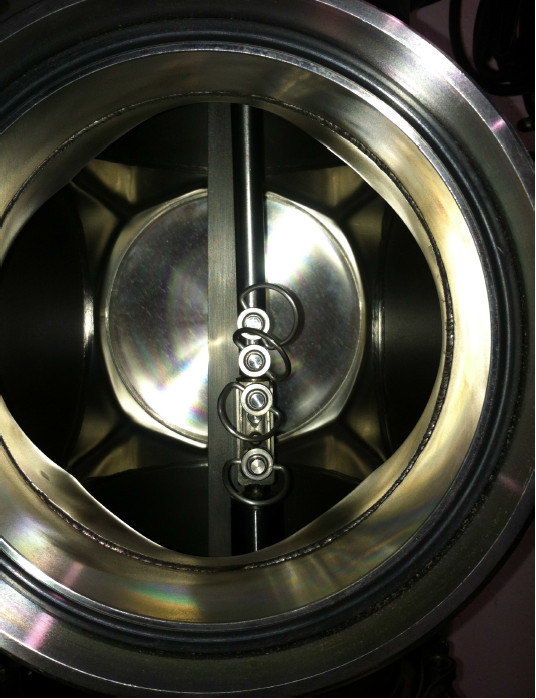
\includegraphics[width=3.2in]{Figures/ArticulationOffset1.jpg}
 \caption{Image of the pig in the home position. The offset of the arm is clearly visible, but below the level that creates problem for motion inside the organ pipe.}
 \label{fig:art_offset1}
\end{figure}

\begin{figure}[htbp]
 \centering
 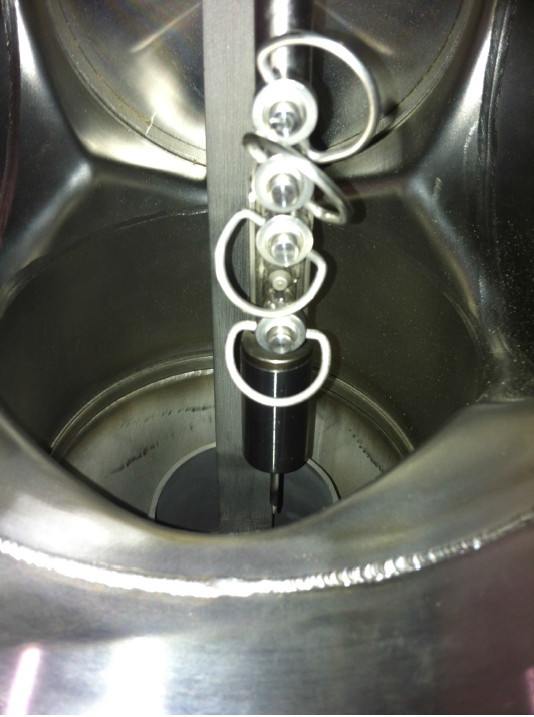
\includegraphics[width=5in]{Figures/ArticulationOffset2.jpg}
 \caption{Another image of the pig in the home position, this time looking down into the lower assembly. Again, note the offset of the arm.}
 \label{fig:art_offset2}
\end{figure}

\begin{figure}[htbp]
 \centering
 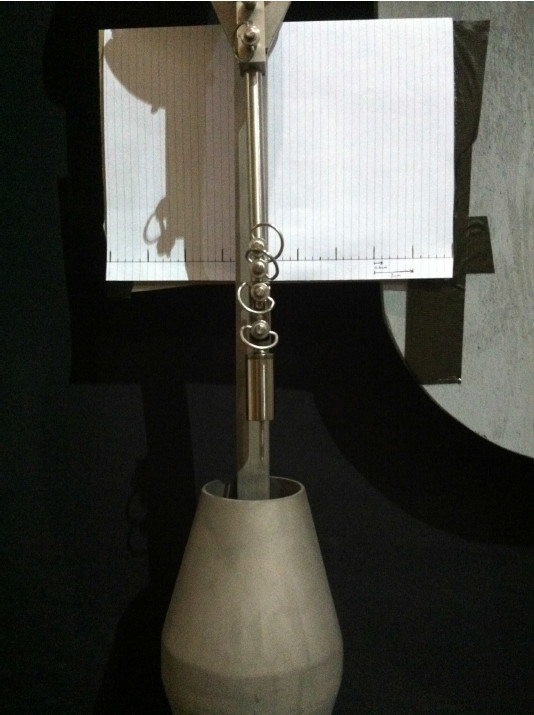
\includegraphics[width=5in]{Figures/ArticulationOffset3.jpg}
 \caption{Image of the pig next to the cryostat mock-up and the ruler used in the horizontal swing test. Note the offset of the arm.}
 \label{fig:art_offset3}
\end{figure}

\begin{figure}[htbp]
 \centering
 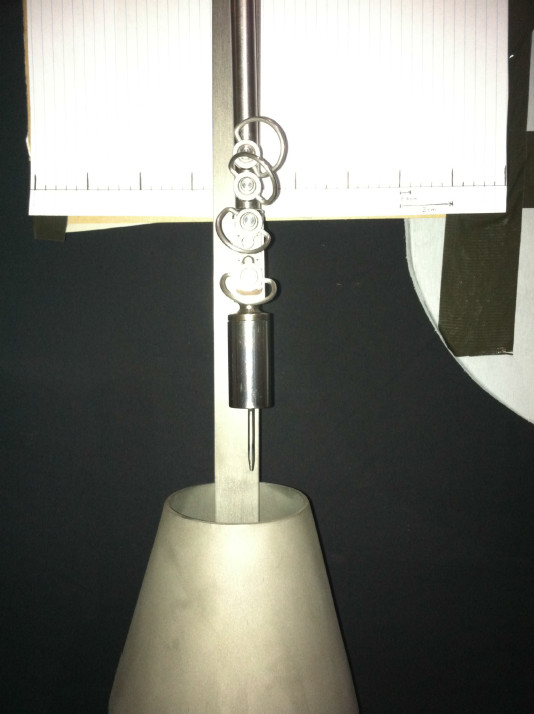
\includegraphics[width=5in]{Figures/ArticulationOffset4.jpg}
 \caption{Again, the pig next to the cryostat mock-up and ruler, a close-up of the arm offset.}
 \label{fig:art_offset4}
\end{figure}

\item{\bf Magnitude of horizontal swing during articulation}

{\bf Procedure:} To measure the horizontal swing of the system during articulation, a 'ruler' was devised and
attached to a mock-up of the cryostat, with a smallest unit of measure of 0.6 cm. The pig was then sent to
the step position where the ruler could be utilized. While the arm was articulated and de-articulated, video
was taken of the swing of the pig.

{\bf Results:}  Anaylsis of the video shows that the pig swings approximately 1.5\,cm during articulation. The articulation is very slow and the swing is very slow. It takes a couple of minutes for the arm to come to complete rest.
    
 \item{Electrical contact test for purpose of determining position of cryostat within the neutron veto}
  
\item{\bf Procedure:} One of the main goals of the first deployment of CALIS-III is to determine the location of the cryostat within the neutron veto as there is a 3-5\,cm positioning uncertainty from construction in the xy-plane and 2\,cm in the z direction.

One test to confirm the position of the cryostat is to electrically connect an arm of the pig to the cryostat. At Fermilab, the electrical contact test was simulated to prove the validity of the idea. The pig was fitted
with a special arm comprised of a stainless steel tube, and the cryostat mock-up received a stainless steel
block attached to it via screws. At the top of CALIS-III, a wire was connected between the lower assembly
and the output of a voltmeter. A wire from the stainless steel block was connected to the voltmeter input. The special arm was first articulated and then the whole assembly was rotated in the azimuthal direction in
order for the arm to make contact with the stainless steel block as can be seen in the Fig.~\ref{fig:electricalContact}.

{\bf Results:} When the arm made contact with the square, the completed circuit was indicated by the
voltmeter. Contact of the arm with the steel block was also verifed by visual inspection. The rotation and
contact was repeated several times and at each contact, the voltmeter registered (by beeping) the connection.

\begin{figure}[htbp]
 \centering
 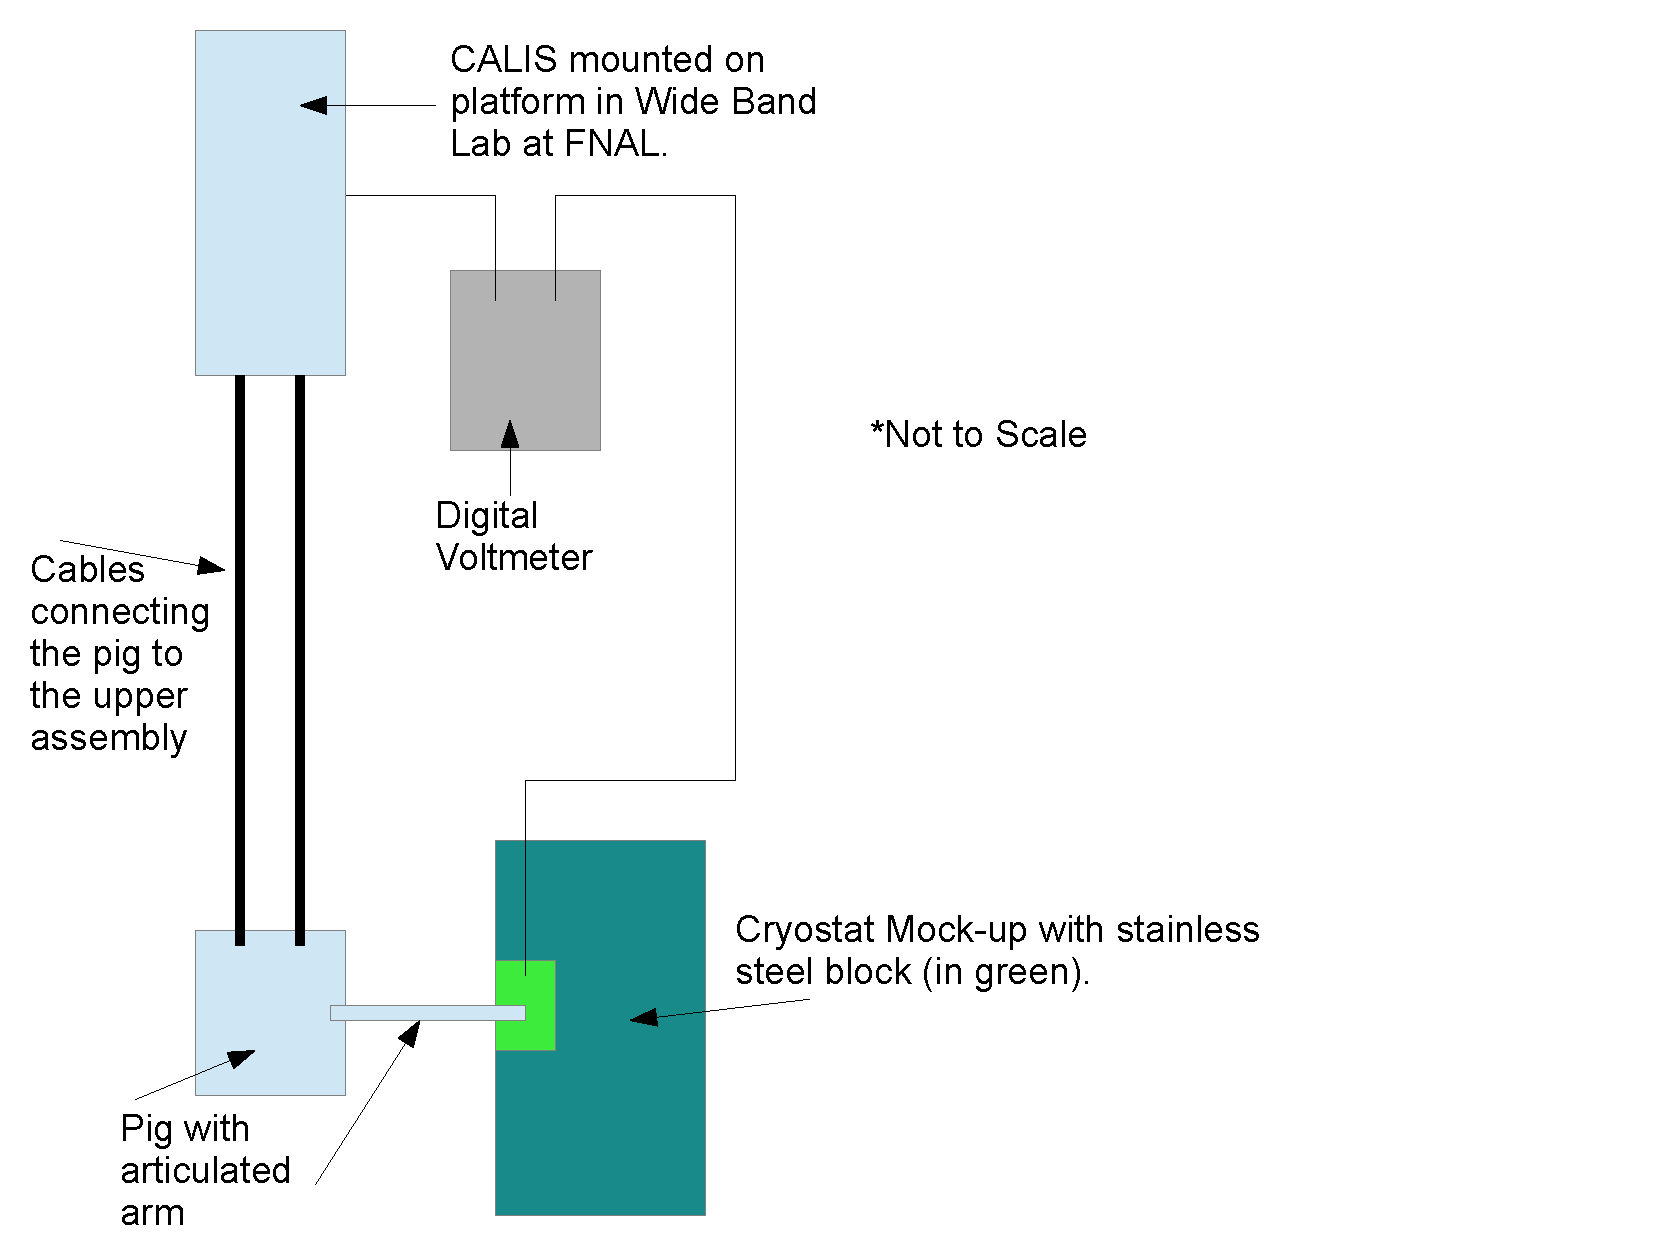
\includegraphics[width=7in]{Figures/electricalContact_FNALtest_diagram}
 \caption{Diagram of the electrical contact test performed at FNAL.}
 \label{fig:electricalContact}
\end{figure}

\item{\bf Functionality of the safety features}

Both the upper limit switch and the arm retraction switch have been tested and operated as expected. 
\begin{itemize}
\item
The pig did not move above the home position, despite the command to move up in z as the power was cut to the motor. 
\item
No z-movement was possible prior to retraction of the arm to the vertical position by the hand wheel. We verify that the arm is vertical by verifying that the dial on the protractor next to the hand wheel is pointing at zero mark. 
\end{itemize}
   
 \item{Test Ease and Accuracy of Azimuthal Rotation}
  
{\bf Procedure:} The upper and lower assemblies of CALIS-III can be rotated in the azimuthal direction.  This rotation allows the source arm to move in the xy plane for the purpose of locating the position of the cryostat within the neutron veto.  The rotation needs to be fairly easy to perform and we need to know what kind of precision and accuracy we will have. The rotation of the upper assembly requires one to loosen the clamp between the upper 
and
lower assembly. Once this is done, the upper assembly is manually moved/twisted on its axis in the direction
desired. To test this at Fermilab, the pig was deployed to the level of the cryostat mock-up and the arm articulated.
Then the clamp was loosened and the upper assembly rotated.

{\bf Results:} Despite its substantial weight, the upper assembly was able to be moved on its axis smoothly,
with no jerking or sticking. At the conclusion of testing, a band was axed to the lower assembly and
a pointer to the band was attached to the upper assembly. This is to measure the actual rotation of the
assembly. Due to time constraints, the rotation with the band attached was not able to be done. Therefore
further testing will need to be done at LNGS to determine the accuracy and precision of the azimuthal
rotation.  
 
\item{Helium Leak Tight Testing}
   
The device was tested to be helium leak tight at Fermilab.  
 
\end{itemize}

 \paragraph{}
  A full summary, along with plots, of the testing performed at Fermilab can be found in DocDB \#858.  

After the above described tests at FNAL were finished, it was concluded that \textit{\bf CALIS is in a good operating state} and is ready to be shipped to LNGS for commissioning and calibration.


\subsection{Commisioning and testing at LNGS}

 The system was shipped sub-assembled to LNGS and arrived in mid-September. Once it arrived, CALIS III was inspected and reasembled. Two rounds of tests are part of the commissioning of CALIS at LNGS: dry tests prior to cleaning and a subset of tests after cleaning the system and prior to installation on the gate valve of CRH. While the goal of the Fermi lab tests was to establish that CALIS is operating as expeced and that all designed safety features are operational, a  goal of the LNGS tests is the final characterization of CALIS to establish the absolute positioning precison of the source. 

The testing location chosen at LNGS allowed full deployment length tests and direct access to both the top of the system where the controls are and to the pig. The chosen locaiton was a tall stairway on the left side of the OPERA detector that has a platform on the fourth floor where CALIS was mounted. A movable platform accessible from the lab floor level was used to raise up to the level of the pig for all planned measurements.   The same set of tests as described above, and a few additional once related to the absolute positioning uncertainty,  have been underway.

 Final characterization of the source positioning must be done with the new cables that have been put on CALIS. The length of the cables was chosen to allow maximum safe, deployment depth that makes any contact with PMTs impossible (according to the engineering drawings of the DarkSide detectors).   Once all dry runs are performed to satisfaction, we will disassemble and clean all components in CR1 as per the normal detector cleaning procedure. After cleaning, the device will be partially assembled and moved into CRH. A subset of validation tests will be conducted from the crane in the CRH and then CALIS will be installed on the top of one of the ate valves.

\subsubsection{Dry Tests to Perform at LNGS Prior to Cleaning}
All the tests performed at Fermilab are  repeated at LNGS, but the number of runs is reduced as we do not expect to see change in the performance of the motor or the cables. While the tests at Fermi lab confirmed good operational performance of the system, the tests conducted at LNGS are calibration tests whose goal is to make the most precise prediction of the source position during deployment and establish expected uncertainty of that position.  Below is the full list of tests underway at LNGS.

 \begin{itemize}
  \item{Characterization of CALIS-III Positioning} 
 
   The CALIS-III positioning has been characterized with the final cables length. There are two components of the positioning: 

\begin{itemize}
\item
This includes the pig z position as a function of step position.
\item 
The arm 90 degree articulation point as a function of vertical pig position.  
\end{itemize}
This is necessary because, as the cable winds around the spool, the winding radius changes, increasing as the pig is lifted and decreasing as it is lowered.  This means that there is not a linear correspondence between the number of steps and the length of cable deployed.  Additionally, this non-linear dependency causes the amount of rotation required by the hand wheel for full articulation of the source arm to change as a function of the length of cable deployed.     
 
  \paragraph{}
  Every 10,000 steps (order of 10\,cm), we stop the pig and record the z position with the laser ranger, as done during the position reproducibility test at Fermilab.  The arm will then be rotated to 90$^{\circ}$ and the hand wheel position noted for the relevant z locations. The step position for key source locations commonly used during calibration will be determined, including the TPC center, 15 cm above and below the TPC center, and the cryostat top and bottom.  Once these positions have been verified by inputting the step location and measuring the z position and corresponding hand wheel rotation, the results will be formatted for easy use by CALIS-III operators.   
  
\item 
Measure the exact distance of the forward motion (in the direction of articulation) at relevant z positions, as it determins the final distance of the source to the TPC.

\item
Measure if there is any lateral change (in the azimuthal plane) when the arm is articulated at relevant z positions. While none has been observed in the previous tests, it is important to verify this in repeated deployments and articulations.

\item 
Validate the distance that the pig moves up during articulation (measured to be 10\,cm in tests at Fermilab) and verify that this number does not change between repeated articulations.

  \item
Test the arm retraction switch to confirm that the pig cannot be retracted to its home position if the arm is articulated.
  
  \item
During articulation measure the level of the horizontal swing. Confirm it to agree with Fermilab testing.
 
  \item{Determine the time it takes for the arm to reach a stable (non-moving) condition after articulation.}
 
  \item{Test the absolute encoder before and after power failure.}
  \item{Test nitrogen and vacuum systems. Measure the amount of time to evacuate the device and purge with nitrogen.}
  \item{Leak check of upper and lower assemblies.}
  \item{Reproducibility of position in x, y, and z following the full procedure.}
 \end{itemize}
 
\subsubsection{Tests to be Performed at LNGS after Cleaning}
 After cleaning of the system, we will attach CALIS-III to a crane either in CR1 or CRH to perform a reduced set of tests.  The goal is to confirm that results from tests prior to cleaning and from after cleaning match. 
  
 
  
\subsection{Proposed Commissioning Plan} \label{Proposed Commissioning Plan}
 \paragraph{}
  Detailed, step by step commissioning procedure is outlined in DocDB\#1021-v1. 
%Once CALIS is installed in CRH, we will need to test gas tightness, light tightness, and evacuation with the vacuum pump.  We will want to move the motors a little bit without opening the gate valve to ensure that all is moving satisfactorily.  Rotation of the whole assembly should be tried at this point and then an alignment will be performed.  We want CALIS to be aligned so that when the arm is articulated it is pointed towards the center of the TPC.  Next, we will open the gate valve and make sure that we can maintain the pressure as it was prior to opening the gate valve.  After that, we will proceed with a 'dummy' deployment (no source in the source holder) down through the organ pipe.  We will start with a low speed and monitor the pressure changes stopping every 5-10 cm to assess the situation.  If all systems are well, then we can increase our descent speed.  At the point of entry into the neutron veto, then we will retract the pig to home position. Once the pig reaches home position, we will again deploy into the neutron veto and attempt articulation of the arm.  We will do the first articulation when we are in optimal viewing from the cameras.  The cameras will be an extra check to ensure that we are at the position that we think we are and be sure we are not going to hit anything.  Once verified, we will dearticulate and continue the deployment, then articulate again when we are near the cryostat and desired testing position.  We will dearticulate and go back to the home position once we are satisfied that the articulation and dearticulation is complete.  As we are lowering CALIS, the DAQ will be monitored to see if there are any electronic noise problems.  We will also monitor to the PMT scalar rates.  By monitoring both the DAQ and the PMT scalars we will be able to tell if there are any light leaks.  
Once all preliminary deployments are completed, we will continue with the cryostat positioning and calibration campaign as outlined in DocDB \#977 for the neutron campaign, DocDB \#978 for the gamma campaign, and DocDB \#960 -- a spreadsheet dedicated to the full campaign.  




\subsection{Source arms}


\textit{My impression is that a drawing to scale with the cryostat, the TPCthe organ pipe and the source arm would be good here}

For articulation, there is currently a choice of three arm lengths---40.31\,cm,  57.15\,cm and 62\,cm.  

Drawing of the arm with the 


Each of these lengths are measured from the center line of the organ pipe to the end of the source holder.  The arm lengths, 57.15\,cm and 62\,cm are intentionally made too long as they will be used to determine the exact location of the cryostat; some uncertainty in the cryostat's z and lateral position exist at the level of 3 - 4\,cm. The organ pipe we intend to use is 81\,cm distant from the cryostat center (and the geometric center of the LSV sphere) as measured from the center line of the organ pipe. The cryostat is 32\,cm in radius, which leaves a distance of $\sim$49\,cm to be reached  by the arm.  The articulation of the arm is operated via a hand wheel located on the side of the upper assembly close to the top.  By rotating the hand wheel, one of the cable spools inside the upper assembly will rotate which pulls up on one of the cables attached to the pig and shortens it for the length equal to the one quarter of the gear curcamference (which is 10\,cm).  As a result, the chain at the bottom of the cables engages the articulation gear (see Fig. \ref{fig:sourcePod_arrows} for an image of the articulation gear) on the pig and raises the arm to horizontal.  The chain has a guard rail that ensures that chain can never come of the gear. Thus, in the process of articulation the entire pig along with the source arm shifts up for 10\,cm.  See Fig. \ref{fig:pigAndCables_fullView} and  Fig. \ref{fig:sourceArmRotation} for a closer look at how CALIS III articulates the arm. In order to determine the degree of articulation of the arm, a protractor is placed next to the hand wheel.  This protractor and the hand wheel are calibrated together for an accurate reading of the articulation. The reading of the protractor dial is different at different heights and calibration table obtained from the tests is used to determine the dial setting necessary to articulate the arm to horizontal position. We have adopted a spherical coordinate system for the rotation of the system and the articulation.  Articulation of the arm is measured in $\theta$ from the z-axis; when the arm is fully articulated, it is at 90$^{\circ}$ and when it is in its vertical position it is at 180$^{\circ}$.  As mentioned in Sec. \ref{The Lower Assembly}, the rotation of CALIS III is done in the xy-plane which corresponds to the azimuthal direction, a rotation in $\phi$.  See Fig. \ref{fig:coordinate_system} for details. 


%%%%%%%%%%%%%%%%%%%%%%%%%%%%%%%%%%%%
\subsection{Calibration of Z-position and Articulation Angle}  